\section{Ablation}
\label{sec:ablation}

Table~\ref{tab:ablation} gives, for each configuration, the held-out false-alarm rate and the detection rate on the stale desk at four lags and on the four other variants, with every configuration calibrated on the same 10,000 null desk-years at a family size of 1\%.
Each row changes one thing from the full complement.

\begin{table}[htbp]
\centering
\footnotesize
\renewcommand{\arraystretch}{1.1}
\caption{Ablation of the complement, first part: held-out false-alarm rate (Size) and detection of the stale-volatility variant at lags of 5, 10, 20 and 40 days (L5 to L40), for the full complement and for each component removed, replaced or changed; every configuration is calibrated on the same 10,000 null desk-years at a family size of 1\% (the no-correction row at 1\% per statistic); percent of 1,000 replications flagged, over the 95\% Wilson interval.}
\label{tab:ablation}
\begin{tabular}{>{\raggedright\arraybackslash}p{3.5cm}ccccc}
\toprule
Configuration & Size & L5 & L10 & L20 & L40 \\
\midrule
Full complement (three statistics, Bonferroni) & \begin{tabular}[t]{@{}c@{}}0.9\\(0.5--1.7)\end{tabular} & \begin{tabular}[t]{@{}c@{}}37.3\\(34.4--40.3)\end{tabular} & \begin{tabular}[t]{@{}c@{}}94.0\\(92.4--95.3)\end{tabular} & \begin{tabular}[t]{@{}c@{}}99.9\\(99.4--100.0)\end{tabular} & \begin{tabular}[t]{@{}c@{}}100.0\\(99.6--100.0)\end{tabular} \\ \addlinespace[0.8ex]
Without the Wald test & \begin{tabular}[t]{@{}c@{}}1.0\\(0.5--1.8)\end{tabular} & \begin{tabular}[t]{@{}c@{}}44.5\\(41.4--47.6)\end{tabular} & \begin{tabular}[t]{@{}c@{}}96.3\\(94.9--97.3)\end{tabular} & \begin{tabular}[t]{@{}c@{}}100.0\\(99.6--100.0)\end{tabular} & \begin{tabular}[t]{@{}c@{}}100.0\\(99.6--100.0)\end{tabular} \\ \addlinespace[0.8ex]
Without the absolute-value Spearman & \begin{tabular}[t]{@{}c@{}}0.6\\(0.3--1.3)\end{tabular} & \begin{tabular}[t]{@{}c@{}}44.4\\(41.3--47.5)\end{tabular} & \begin{tabular}[t]{@{}c@{}}96.3\\(94.9--97.3)\end{tabular} & \begin{tabular}[t]{@{}c@{}}99.9\\(99.4--100.0)\end{tabular} & \begin{tabular}[t]{@{}c@{}}100.0\\(99.6--100.0)\end{tabular} \\ \addlinespace[0.8ex]
Without the rolling-mean Spearman & \begin{tabular}[t]{@{}c@{}}1.0\\(0.5--1.8)\end{tabular} & \begin{tabular}[t]{@{}c@{}}3.8\\(2.8--5.2)\end{tabular} & \begin{tabular}[t]{@{}c@{}}17.3\\(15.1--19.8)\end{tabular} & \begin{tabular}[t]{@{}c@{}}67.7\\(64.7--70.5)\end{tabular} & \begin{tabular}[t]{@{}c@{}}92.4\\(90.6--93.9)\end{tabular} \\ \addlinespace[0.8ex]
Wald test alone & \begin{tabular}[t]{@{}c@{}}0.8\\(0.4--1.6)\end{tabular} & \begin{tabular}[t]{@{}c@{}}2.4\\(1.6--3.5)\end{tabular} & \begin{tabular}[t]{@{}c@{}}6.0\\(4.7--7.6)\end{tabular} & \begin{tabular}[t]{@{}c@{}}14.2\\(12.2--16.5)\end{tabular} & \begin{tabular}[t]{@{}c@{}}28.7\\(26.0--31.6)\end{tabular} \\ \addlinespace[0.8ex]
Absolute-value Spearman alone & \begin{tabular}[t]{@{}c@{}}1.6\\(1.0--2.6)\end{tabular} & \begin{tabular}[t]{@{}c@{}}4.5\\(3.4--6.0)\end{tabular} & \begin{tabular}[t]{@{}c@{}}25.6\\(23.0--28.4)\end{tabular} & \begin{tabular}[t]{@{}c@{}}76.7\\(74.0--79.2)\end{tabular} & \begin{tabular}[t]{@{}c@{}}94.1\\(92.5--95.4)\end{tabular} \\ \addlinespace[0.8ex]
Rolling-mean Spearman alone (20 days) & \begin{tabular}[t]{@{}c@{}}1.2\\(0.7--2.1)\end{tabular} & \begin{tabular}[t]{@{}c@{}}57.6\\(54.5--60.6)\end{tabular} & \begin{tabular}[t]{@{}c@{}}97.5\\(96.3--98.3)\end{tabular} & \begin{tabular}[t]{@{}c@{}}99.9\\(99.4--100.0)\end{tabular} & \begin{tabular}[t]{@{}c@{}}100.0\\(99.6--100.0)\end{tabular} \\ \addlinespace[0.8ex]
Rolling-mean Spearman, 5 days & \begin{tabular}[t]{@{}c@{}}1.2\\(0.7--2.1)\end{tabular} & \begin{tabular}[t]{@{}c@{}}91.1\\(89.2--92.7)\end{tabular} & \begin{tabular}[t]{@{}c@{}}99.8\\(99.3--99.9)\end{tabular} & \begin{tabular}[t]{@{}c@{}}100.0\\(99.6--100.0)\end{tabular} & \begin{tabular}[t]{@{}c@{}}100.0\\(99.6--100.0)\end{tabular} \\ \addlinespace[0.8ex]
Rolling-mean Spearman, 10 days & \begin{tabular}[t]{@{}c@{}}1.0\\(0.5--1.8)\end{tabular} & \begin{tabular}[t]{@{}c@{}}82.9\\(80.4--85.1)\end{tabular} & \begin{tabular}[t]{@{}c@{}}99.8\\(99.3--99.9)\end{tabular} & \begin{tabular}[t]{@{}c@{}}100.0\\(99.6--100.0)\end{tabular} & \begin{tabular}[t]{@{}c@{}}100.0\\(99.6--100.0)\end{tabular} \\ \addlinespace[0.8ex]
Rolling-mean Spearman, 40 days & \begin{tabular}[t]{@{}c@{}}1.0\\(0.5--1.8)\end{tabular} & \begin{tabular}[t]{@{}c@{}}24.2\\(21.6--27.0)\end{tabular} & \begin{tabular}[t]{@{}c@{}}83.4\\(81.0--85.6)\end{tabular} & \begin{tabular}[t]{@{}c@{}}98.4\\(97.4--99.0)\end{tabular} & \begin{tabular}[t]{@{}c@{}}99.9\\(99.4--100.0)\end{tabular} \\ \addlinespace[0.8ex]
Rolling-mean Spearman, 60 days & \begin{tabular}[t]{@{}c@{}}1.0\\(0.5--1.8)\end{tabular} & \begin{tabular}[t]{@{}c@{}}15.4\\(13.3--17.8)\end{tabular} & \begin{tabular}[t]{@{}c@{}}61.9\\(58.8--64.9)\end{tabular} & \begin{tabular}[t]{@{}c@{}}94.2\\(92.6--95.5)\end{tabular} & \begin{tabular}[t]{@{}c@{}}98.8\\(97.9--99.3)\end{tabular} \\ \addlinespace[0.8ex]
OLS covariance in place of HC3 & \begin{tabular}[t]{@{}c@{}}1.1\\(0.6--2.0)\end{tabular} & \begin{tabular}[t]{@{}c@{}}44.2\\(41.1--47.3)\end{tabular} & \begin{tabular}[t]{@{}c@{}}95.4\\(93.9--96.5)\end{tabular} & \begin{tabular}[t]{@{}c@{}}100.0\\(99.6--100.0)\end{tabular} & \begin{tabular}[t]{@{}c@{}}100.0\\(99.6--100.0)\end{tabular} \\ \addlinespace[0.8ex]
No multiplicity correction (1\% each) & \begin{tabular}[t]{@{}c@{}}3.3\\(2.4--4.6)\end{tabular} & \begin{tabular}[t]{@{}c@{}}59.4\\(56.3--62.4)\end{tabular} & \begin{tabular}[t]{@{}c@{}}97.9\\(96.8--98.6)\end{tabular} & \begin{tabular}[t]{@{}c@{}}100.0\\(99.6--100.0)\end{tabular} & \begin{tabular}[t]{@{}c@{}}100.0\\(99.6--100.0)\end{tabular} \\ \addlinespace[0.8ex]
Rolling means at 5, 10, 20 and 40 days (Bonferroni) & \begin{tabular}[t]{@{}c@{}}0.5\\(0.2--1.2)\end{tabular} & \begin{tabular}[t]{@{}c@{}}76.7\\(74.0--79.2)\end{tabular} & \begin{tabular}[t]{@{}c@{}}99.5\\(98.8--99.8)\end{tabular} & \begin{tabular}[t]{@{}c@{}}100.0\\(99.6--100.0)\end{tabular} & \begin{tabular}[t]{@{}c@{}}100.0\\(99.6--100.0)\end{tabular} \\ \addlinespace[0.8ex]
Full complement and regulatory zone & \begin{tabular}[t]{@{}c@{}}0.9\\(0.5--1.7)\end{tabular} & \begin{tabular}[t]{@{}c@{}}37.3\\(34.4--40.3)\end{tabular} & \begin{tabular}[t]{@{}c@{}}94.0\\(92.4--95.3)\end{tabular} & \begin{tabular}[t]{@{}c@{}}99.9\\(99.4--100.0)\end{tabular} & \begin{tabular}[t]{@{}c@{}}100.0\\(99.6--100.0)\end{tabular} \\ \addlinespace[0.8ex]
\bottomrule
\end{tabular}
\end{table}


\subsection{What each component contributes}
\label{sec:ablation-components}

Removing the rolling-mean statistic costs the stale-volatility detection: from 37.3, 94.0, 99.9 and 100.0\% at lags of 5, 10, 20 and 40 days to 3.8, 17.3, 67.7 and 92.4\%.
It is the component that carries the result, and it carries it alone: the rolling-mean statistic on its own flags 57.6, 97.5, 99.9 and 100.0\% at its own 1\% size.
Removing the absolute-value statistic costs little on the six variants (the stale detection is unchanged within 0.1 points at 20 days, and the omitted-factor detection falls from 100.0 to 97.3\%), because the rolling-mean statistic and the Wald statistic cover most of what it sees; its single-statistic row shows what it sees alone: 76.7\% at a lag of 20 days, 100.0\% of the missing-basis variant, which the Wald statistic cannot see, and 100.0\% of the omitted-factor variant.
Removing the Wald statistic drops the wrong-correlation detection from 100.0 to 7.4\%, and the only other change is the gain at short lags that the smaller multiplicity split brings (44.5 against 37.3\% at 5 days and 96.3 against 94.0\% at 10); the Wald statistic alone flags the wrong correlation and the time misalignment (100.0\% each) and is blind to the missing basis (0.9\%) and the omitted factor (0.6\%), as the theory predicts.
The regulatory zone flags the wrong correlation and the time misalignment in 100.0\% of replications, so on these six variants the Wald statistic adds nothing that the zone does not already provide; its unique contribution is the constant mis-scale of Table~\ref{tab:mis-scale}, which neither the zone nor the rank statistics see.
Adding the regulatory zone to the union changes no rate in the table, since the zone flags none of the stale desks.
The multiplicity split has a price: with three statistics each at 0.333\% the detection at a lag of 5 days is 37.3\%, and with two statistics (the rows without the Wald or the absolute-value statistic) it is 44.5 and 44.4\%.

\subsection{The window}
\label{sec:ablation-window}

The rolling window was fixed at 20 days before the evaluation, and Table~\ref{tab:ablation} and Figure~\ref{fig:window-ablation} show how the rate depends on it.
At equal size (between 1.0 and 1.2\% held out for every window) shorter windows detect more of the short lags: at a lag of 5 days the rate is 91.1\% for a window of 5 days, 82.9\% for 10, 57.6\% for 20, 24.2\% for 40 and 15.4\% for 60; at a lag of 10 days it is 99.8, 99.8, 97.5, 83.4 and 61.9\%.
Shorter windows also hold the time-misalignment detection (100.0\% at 5 days and 94.5\% at 10, against 42.3\% at 20 and 5.3\% at 60), because a one-day shift of the series is visible in a rolling mean only when the mean is short.
No window helps against the wrong correlation (2.6 to 8.9\%), which is a defect of the cross-sectional aggregation and not of the scale.
Combining four windows (5, 10, 20 and 40 days) by a Bonferroni split over four statistics gives 76.7\% at a lag of 5 days and 99.5\% at 10, at a held-out size of 0.5\% (0.2 to 1.2\%), between the best single window and the default.
The window of 20 days is therefore not the best of the windows tested on these desks.
It is kept as the method's default because it was fixed in advance and because this table was computed on the same committed seeds as the main results: choosing the best window from it would select on the evaluation data, and a change of the default needs an evaluation on desks that this table has not seen.

\begin{figure}[htbp]
\centering
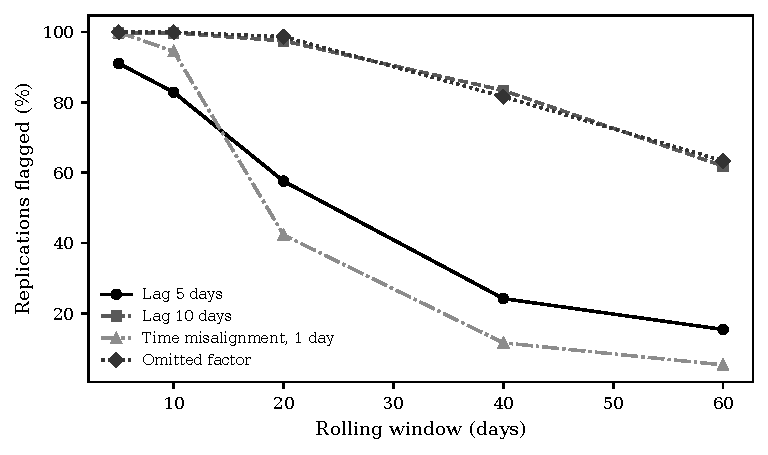
\includegraphics[width=0.86\linewidth]{window-ablation}
\caption{Percent of 1,000 replications flagged by the rolling-mean Spearman statistic against the length of its window in days, at a size of 1\% read from the 10,000 null desk-years, on the stale-volatility desk at lags of 5 and 10 days and on the time-misalignment and omitted-factor variants.}
\label{fig:window-ablation}
\end{figure}

\subsection{The covariance and the multiplicity correction}
\label{sec:ablation-covariance}

The HC3 covariance is motivated by the time-varying volatility of the profit and loss (Section~\ref{sec:method-regression}), and the ablation tests whether it earns its place in the decision.
Replacing it by the ordinary least-squares covariance in the three-statistic union gives a held-out size of 1.1\% against 0.9\% and detection rates of 44.2, 95.4, 100.0 and 100.0\% at lags of 5, 10, 20 and 40 days, against 37.3, 94.0, 99.9 and 100.0\%; the Wald statistic alone flags the stale desk in 41.0\% of replications with the ordinary covariance and in 14.2\% with HC3.
The decision never uses the asymptotic $\chi^2_2$ reference, because its threshold is read from the simulated null, which absorbs the heteroskedasticity either way; the HC3 covariance then gives no gain in power on these desks and costs some, and the choice is kept only because it makes the reference p-value that the engine reports meaningful on a desk whose volatility is not constant.
This is a negative result for the HC3 component of the specification as it stands: a decision read only from the simulated null does not need it.
Removing the multiplicity correction, so that each statistic is calibrated at 1\%, raises the detection at a lag of 5 days from 37.3 to 59.4\% and the held-out size from 0.9\% to 3.3\% (2.4 to 4.6\%), which is the size that three statistics at 1\% each allow; the Bonferroni split keeps the stated family size at the price of about 22 points of power at the shortest lag and none at a lag of 20 days.
